\chapter{NP-completezza} \label{ch:capitolo12}
\subsection{P = NP?}
\begin{itemize}
    \item\textbf{P} 
    
è la classe dei problemi che ammettono un algoritmo di decisione rapido (= polinomiale)
    
    \item\textbf{NP} 
    
è la classe dei problemi che ammettono un algoritmo di verifica rapido (= polinomiale)
\end{itemize}
Quindi P $\subseteq$ NP significa la verifica è più rapida della decisione.\\
Ma P = NP significherebbe che se c’è una procedura rapida di verifica per S, ce n’è una di decisione, veloce anch’essa. 
\begin{itemize}
    \item P è la classe dei problemi accettati da macchine di Turing deterministiche in tempo polinomiale
    
    \item NP è la classe dei problemi accettati da macchine di Turing non deterministiche in tempo polinomiale
\end{itemize}
Ogni macchina di Turing non deterministica è simulata da una macchina di Turing deterministica, ma la complessità cresce esponenzialmente. Si può fare meglio?\\\\\\
\textbf{Osservazione}\\
Se trovo un problema S di classe NP che non sta in P, allora P $\neq$ NP, Per dimostrare P = NP, dovrei dimostrare che tutti i problemi S $\in$ NP sono di classe P.
Vedremo invece che esiste una famiglia di problemi di classe NP (tra i quali, p.es., SAT) tale che se anche uno solo di essi appartiene a P, allora P = NP.
\subsection{Riduzioni polinomiali}
\textbf{Definizione}\\
Siano S, T due problemi su alfabeti A, B, rispettivamente.\\
Una riduzione polinomiale di S a T è una funzione totale $f : A^* \mapsto B^*$ tale che
\begin{figure}[htp]
    \centering
    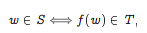
\includegraphics[scale=0.9]{tesi_stile/img/foto1cap12.png}
\end{figure}
calcolata da una macchina di Turing deterministica con complessità temporale polinomiale.
Se esiste una riduzione polinomiale di S a T, scriveremo $S <=_p T$.\\\\
\textbf{Osservazione}\\
La relazione $<=_p$ è riflessiva e transitiva (pre-ordine).\\\\
\textbf{Esempio}\\
2COL $<=_p$ 2SAT, IS $<=_p$ CLIQUE $<=_p$ VC $<=_p$ IS.\\\\
\textbf{Proposizione}\\
Siano S, T due problemi. Se S $<=_p$ T e T $\in$ P (risp., T $\in$ NP), allora S $\in$ P (risp., S $\in$ NP).
\newpage
\subsection{Problemi NP-ardui}
\textbf{Definizione}\\
Un problema T si dice NP-arduo se, per ogni S $\in$ NP si ha S $<=_p$ T.
Un problema T si dice NP-completo se è NP-arduo e appartiene alla classe
NP.\\\\
\textbf{Proposizione}\\
Sia S un problema NP-completo. Se S $\in$ P, allora P = NP.
\subsection{Un problema NP-completo}
Si consideri il seguente problema LHalt:\\\\
\textbf{Input:} una macchina di Turing non deterministica M, un input w di
M, un’altra parola u;\\
\textbf{Output:} SI se una computazione di M converge su w in al più l(u) passi, NO altrimenti.\\\\
\textbf{Proposizione}\\
Si ha LHalt $\in$ NP.\\\\
\textbf{Dimostrazione}\\
Il problema è accettato dalla seguente procedura non deterministica in
tempo polinomiale:
\begin{enumerate}
    \item calcolare k = l(u)
    
    \item eseguire (non deterministicamente) M su w per un massimo di k passi; se M non si arresta, proseguire con un ciclo infinito.
\end{enumerate}
\textbf{Proposizione}\\
Il problema LHalt è NP-arduo\\\\
\textbf{Dimostrazione}\\
Sia S $\in$ NP. Allora esiste una macchina di Turing non deterministica M che accetta S e tale che
\begin{center}
    $c_M(n) <= P(n)$
\end{center}
per un opportuno polinomio P. La funzione f definita da
\begin{figure}[htp]
    \centering
    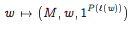
\includegraphics[scale=0.9]{tesi_stile/img/foto2cap12.png}
\end{figure}
è una riduzione polinomiale di S a LHalt.\\
Data l’arbitrarietà di S, possiamo concludere che LHalt è NP-arduo.
Dalle proprietà precedenti segue immediatamente che\\\\
\textbf{Corollario}\\
LHalt è NP-completo.
\subsection{Il teorema di Cook-Levin}
\textbf{Teorema (Cook-Levin, 1971)}\\
SAT è NP-completo.\\\\
\textbf{Proposizione}\\
Si ha SAT $\in$ NP.\\\\
\textbf{Dimostrazione}\\
L’insieme
\begin{figure}[htp]
    \centering
    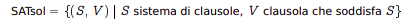
\includegraphics[scale=0.9]{tesi_stile/img/foto3cap12.png}
\end{figure}
è di classe P e si ha S $\in$ SAT $\Longleftrightarrow$(S,V) $\in$ SATsol per un opportuno V.
\newpage
\textbf{Proposizione}\\
SAT è NP-arduo.\\\\
\textbf{Dimostrazione}\\
Sia S $\in$ NP. Allora esiste una macchina di Turing non deterministica M che
\begin{center}
    $c_M(n) <= p(n)$
\end{center}
per un opportuno polinomio p.
Costruiremo una riduzione polinomiale di S a SAT.
\newpage
\section{Il Teorema di Cook-Levin - Approfondito}
Si consideri il seguente problema LHalt:\\
\textbf{INPUT:} una macchina di Turing non deterministica M, un input w di M, un’altra parola u;\\
\textbf{OUTPUT:} SI se M converge su w in al più l(u) passi, NO altrimenti.\\
Vedremo che LHalt è un problema NP-completo.\\\\
\textbf{Proposizione 1}\\ 
Si ha LHalt $\in$ NP.\\\\
\textbf{DIMOSTRAZIONE}\\ 
Una procedura non deterministica che accetta LHalt in tempo polinomiale è la seguente:
\begin{enumerate}
    \item calcolare k = l(u)
    \item eseguire (non deterministicamente) M su w per un massimo di k passi; se M non si arresta, proseguire con un ciclo infinito.
\end{enumerate}
Chiaramente, si ha (M, w, u) $\in$ LHalt se e solo se una delle possibili esecuzioni della suddetta procedura termina. \\Poiché la simulazione è limitata a k = l(u) passi, la classe di complessità è NP.\\
\\\textbf{Proposizione 2}
\\Il problema LHalt è \textbf{NP-arduo.}
\\\textbf{DIMOSTRAZIONE} 
\\Sia S $\in$ NP. Allora esiste una macchina di Turing non deterministica M che accetta S e tale che 
\begin{center}
    $c_M(n) <= P(n)$
\end{center}
per un opportuno polinomio P. La funzione f definita da:
\begin{center}
    $w  \mapsto , w, 1^{P(l(w)})$
\end{center}
è una riduzione di S a LHalt. Il calcolo di tale funzione si riduce al calcolo di $k = P(l(w))$ e alla concatenazione di M, w e $1^k$. Si calcola pertanto in tempo costante. Data l’arbitrarietà di S, possiamo concludere che ogni problema di classe NP si riduce a LHalt in tempo polinomiale (anzi, costante). Questo dimostra che LHalt è
NP-arduo.
\\Dalle proprietà precedenti segue immediatamente che\\\\
\textbf{Corollario 1}\\ 
LHalt è NP-completo.\\
Vedremo ora un esempio ‘naturale’ di problema NP-completo.\\\\
\textbf{Teorema 1 (Cook-Levin, 1971)}
\\SAT è NP-completo. Per dimostrare il Teorema di Cook-Levin dobbiamo verificare che SAT $\in$ NP (Proposizione 3) e che è un problema NP-arduo (Proposizione 4).\\\\
\textbf{Proposizione 4}
\\SAT è NP-arduo.\\\\
\textbf{Dimostrazione}\\
Sia S $\in$ NP. Allora esiste una macchina di Turing non deterministica M che accetta S e tale che
\begin{center}
    $c_M(n) <= p(n)$
\end{center}
per un opportuno polinomio p.\\
Detti Q, A e I rispettivamente l’alfabeto, l’insieme degli stati e l’insieme delle istruzioni di M, poniamo
\begin{center}
    $A = \{a_0, a_1,..., a_m\} , Q = \{q_0, q_1,..., q_h\} , I = \{\alpha_0, \alpha_1,..., \alpha_l\}$
\end{center}
con $a_0 = \#, m, h, l >= 0$. Senza perdita di generalità, possiamo ridurci al caso in cui M si arresta se e solo se entra nello stato $q_h$. Possiamo inoltre supporre che risulti
\begin{center}
    $p(n) >= n$
\end{center}
per ogni $n>=0$
Passiamo ora alla costruzione di una riduzione di S a SAT. Dobbiamo costruire una funzione totale f che associa a ogni parola w $\in$ $A^*$ un sistema di clausole f(w) in modo tale che f(w) sia soddisfacibile se e solo se w $\in$ S. Evidentemente, tale sistema dovrà in qualche modo 'rappresentare' le computazioni di M.\\
Poniamo T = p(l(w)). È possibile associare un indice a ogni cella del nastro di M nel modo seguente:
\\ la cella in cui si trova inizialmente la testina ha indice 0, quella alla sua destra 1, la successiva 2, e così via, mentre le celle alla sinistra della cella di indice 0 avranno gli indici -1, -2, ecc
\begin{figure}[htp]
    \centering
    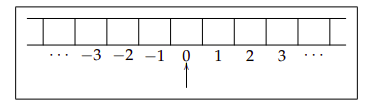
\includegraphics[scale=0.6]{tesi_stile/img/levin1.png}
\end{figure}
Si osservi che in una computazione che duri non più di T passi, la testina potrà
visitare solo le celle di indice compreso tra -T e T. Potremo quindi disinteressarci delle celle al di fuori di tale intervallo.
\\Definiamo i letterali del nostro sistema e contemporaneamente una valutazione, detta valutazione standard associata a una generica computazione di M.
\begin{figure}[htp]
    \centering
    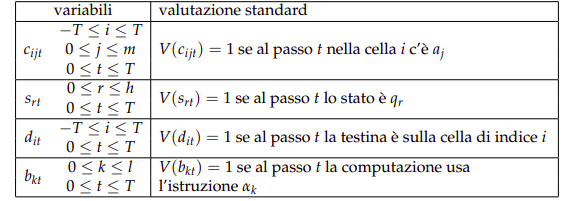
\includegraphics[scale=0.6]{tesi_stile/img/levin2.png}
\end{figure}
Ora cerchiamo di costruire il nostro sistema f(w) in modo tale che sia soddisfatto
esclusivamente dalle valutazioni standard delle computazioni di M. Iniziamo introducendo le clausole.
\begin{figure}[htp]
    \centering
    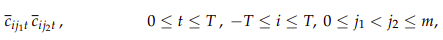
\includegraphics[scale=0.6]{tesi_stile/img/levin3.png}
\end{figure}
\\Una valutazione V soddisfa tali clausole se e solo se comunque fissati i e t c’è al più un indice j per cui $V_{(cijt)} = 1$. 
\newpage
Ora aggiungiamo al nostro sistema le clausole
\begin{figure}[htp]
    \centering
    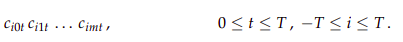
\includegraphics[scale=0.6]{tesi_stile/img/levin4.png}
\end{figure}
\\Una valutazione V soddisfa tali clausole se e solo se comunque fissati i e t c’è almeno
un indice j per cui $V_{(cijt)} = 1$. In conclusione una valutazione V soddisfa le clausole precedenti se e solo se per ogni i e t, esiste uno e un solo j tale che $V_{(cijt)} = 1$. In altri termini, tale condizione esprime il fatto che a ogni passo di una computazione di una macchina di Turing ogni cella del nastro contiene una e una sola lettera.
\\Allo stesso modo, aggiungiamo al nostro sistema le clausole.\\
Aggiungiamo ancora le clausole\\
\begin{figure}[htp]
    \centering
    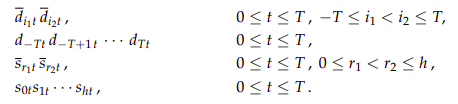
\includegraphics[scale=0.6]{tesi_stile/img/levin5.png}
\end{figure}
\\Tali clausole assicurano che se V è una valutazione che soddisfa il sistema, allora, per ogni t, ci sono esattamente un indice i e un indice r tale che $V_{(dit)} = 1$ e $V_{(srt)} = 1$.
\\In altri termini queste clausole esprimono l’unicità della posizione della testina e dello stato a ogni istante di una computazione di una macchina di Turing. 
\\Aggiungiamo ancora le clausole
\begin{figure}[htp]
    \centering
    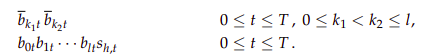
\includegraphics[scale=0.6]{tesi_stile/img/levin6.png}
\end{figure}
\newpage
Tali clausole assicurano che se V è una valutazione che soddisfa il sistema, allora, per qualsiasi t tale che $V_{(sht)} = 0$, c’è esattamente un indice k tale che $V_{(bkt)} = 1$. Ciò esprime il fatto che una MdT applica un’unica istruzione a ogni passo di computazione fino a un eventuale arresto. Introduciamo ora le clausole che esprimono il fatto che il contenuto di una cella non viene modificato quando la testina non si trova su quella cella. \\Ciò si ottiene con le clausole
\begin{figure}[htp]
    \centering
    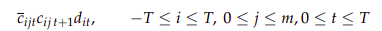
\includegraphics[scale=0.6]{tesi_stile/img/levin7.png}
\end{figure}
\\Inoltre per ogni istruzione$ \alpha_k =(q_{r1}, a_{j1}, q_{r2}, a_{j2}, \epsilon), 0 <= k <= l$, introduciamo le clausole:
\begin{figure}[htp]
    \centering
    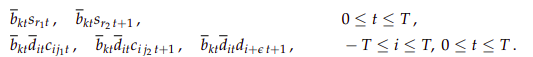
\includegraphics[scale=0.6]{tesi_stile/img/levin8.png}
\end{figure}
Tali clausole esprimono il fatto che lo stato, il contenuto della cella sotto la testina e la
posizione della testina cambiano in accordo con l’istruzione utilizzata all’istante t.
Ancora posto $w = a_{j0},a_{j1},...,a_{jn-1}$, introduciamo le clausole
\begin{figure}[htp]
    \centering
    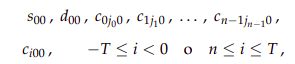
\includegraphics[scale=0.6]{tesi_stile/img/levin9.png}
\end{figure}
che esprimono le condizioni iniziali della computazione e la clausola
\begin{center}
    $s_{h0},s_{h1},...,s_{hT}$
\end{center}
che esprime il fatto che la computazione si arresta in tempo $<= T$.
\\Dalla costruzione segue che una valutazione V soddisfa f(w) se e solo se V è la valutazione standard associata a una computazione di M su w che converge in non più di T passi. Ne segue che w $\in$ S se e solo se f(w) $\in$ SAT. Quindi f è una riduzione di S a SAT. Osserviamo poi che f(w) è costituito da $O(T^2)$ clausole ciascuna di lunghezza
O(T). Ne segue che il calcolo di f richiede tempo polinomiale. Possiamo così concludere che S $<=_p$ SAT.
\\Data l’arbitrarietà di S, abbiamo dimostrato che ogni problema di classe NP si riduce a SAT in tempo polinomiale. Questo dimostra che SAT è NP-arduo











\newpage
\subsection{Riduzione di S e SAT}
Siano
\begin{center}
    A = $\{a_0,a_1,..., a_m \}$ , Q = $\{q_0, q_1,...,q_h \}$ , I = ${\alpha_0, \alpha_1,..., \alpha_l}$.
\end{center}
rispettivamente l’alfabeto, l’insieme degli stati e l’insieme delle istruzioni di M, con $a_0 = \#$.\\
Possiamo supporre che M si arresta se e solo se entra nello stato $q_h$ e che $p(n) >= n$, per ogni $n >= 0$.\\
Dobbiamo costruire una funzione totale f che associa a ogni parola w $\in$ A* un sistema di clausole f(w) in modo tale che f(w) sia soddisfacibile se e solo se w $\in$ S.\\
Faremo in modo di ‘rappresentare’ le computazioni di M nelle clausole.\\\\
Poniamo T = p(l(w))
\begin{figure}[htp]
    \centering
    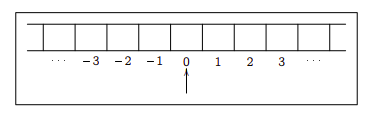
\includegraphics[scale=0.9]{tesi_stile/img/foto4cap12.png}
\end{figure}
\subsection{Variabili}
Definiamo le variabili del nostro sistema e contemporaneamente una
valutazione, detta valutazione standard associata a una generica
computazione di M.
\begin{figure}[htp]
    \centering
    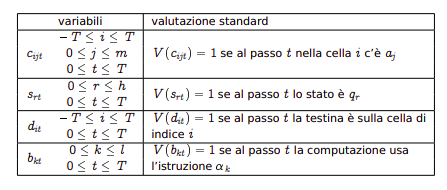
\includegraphics[scale=0.9]{tesi_stile/img/foto5cap12.png}
\end{figure}
\subsection{Clausole}
Costruiamo il sistema f (w) in modo tale che sia soddisfatto esclusivamente dalle valutazioni standard delle computazioni convergenti di M.
\begin{figure}[htp]
    \centering
    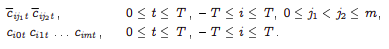
\includegraphics[scale=0.9]{tesi_stile/img/foto6cap12.png}
\end{figure}
sono soddisfatte se e solo se per ogni i e t c’è uno e un solo j tale che $V(c_{ijt}) = 1$: ogni cella, a ogni istante contiene una e una sola lettera.
\begin{figure}[htp]
    \centering
    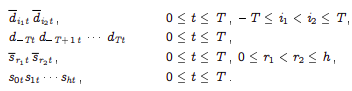
\includegraphics[scale=0.9]{tesi_stile/img/foto7cap12.png}
\end{figure}
a ogni istante c’è un’unica la posizione della testina e un unico stato.
\section{Altre clausole}
\begin{figure}[htp]
    \centering
    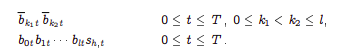
\includegraphics[scale=0.9]{tesi_stile/img/foto8cap12.png}
\end{figure}
(un’unica istruzione a ogni passo di computazione, fino a un eventuale
arresto).\\
Per ogni istruzione $a_k$ = $(q_{r1}, a_{j1}, q_{r2}, a_{j2}, \epsilon)$, $0 <= k <= l$, introduciamo le
clausole:
\begin{figure}[htp]
    \centering
    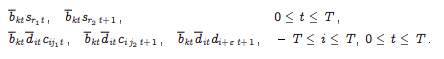
\includegraphics[scale=0.9]{tesi_stile/img/foto9cap12.png}
\end{figure}
(all’istante t lo stato, il contenuto della cella sotto la testina e la posizione della testina cambiano in accordo con l’istruzione $\alpha_t$)
\begin{figure}[htp]
    \centering
    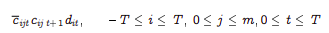
\includegraphics[scale=0.9]{tesi_stile/img/foto10cap12.png}
\end{figure}
(nessun’altra cella è modificata).
\newpage
\subsection{Ancora clausole}
\begin{figure}[htp]
    \centering
    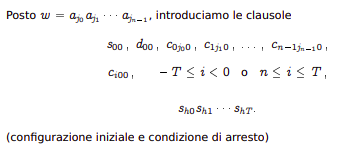
\includegraphics[scale=0.9]{tesi_stile/img/foto11cap12.png}
\end{figure}
\subsection{Conclusione}
\begin{itemize}
    \item Una valutazione V soddisfa f (w) se e solo se V è la valutazione standard associata a una computazione di M su w che converge in al più T passi.
    
    \item Quindi w $\in$ S $\Longleftrightarrow$ f(w) $\in$ SAT.
    
    \item Ci sono $O(T^2)$ clausole ciascuna di lunghezza O(T). Quindi f si calcola in tempo polinomiale
    
    \begin{center}
        S $<=_p$ SAT.
    \end{center}
    
    \item SAT è NP-arduo.
\end{itemize}